\documentclass[12pt]{article}

\usepackage{amsmath}
\usepackage{graphicx}
\usepackage{caption}
\usepackage{subcaption}
\usepackage{enumerate}
\usepackage{rotating}
\usepackage{multirow}
\usepackage{booktabs}
\usepackage{parskip}
\usepackage{setspace}
\usepackage{dcolumn}
\usepackage{hyperref}
\hypersetup{pdfstartpage=1,
            pdfpagemode=UseNone,
            pdfstartview=FitH,
            pdffitwindow=true,
            bookmarks=false,
            colorlinks=true,
            urlcolor=blue,
            linkcolor=blue,
            citecolor=blue}
\usepackage[top=1in,bottom=1in,left=1in,right=1in]{geometry}
\usepackage{lastpage}
\usepackage{fancyhdr}
\usepackage{afterpage}

\pagestyle{fancy}
\fancyhead{} % clear all header fields
\fancyfoot{} % clear all footer fields
\fancyhead[L]{Latner}
\fancyhead[C]{Income volatility and mobility}
\fancyhead[R]{Page \thepage\  of \pageref*{LastPage}}
\renewcommand{\headrulewidth}{0pt}
\renewcommand{\footrulewidth}{0pt}

\fancypagestyle{firststyle}
{
   \fancyhead{}
   \fancyfoot{}
}

\begin{document}

\begin{center}
\large Income volatility and mobility: A conceptual exploration of two frameworks \\
\bigskip
\normalsize
Jonathan P. Latner $^{a}$\\
\end{center}

{\bf  Abstract}

This paper explores two frameworks for measuring income volatility using data from the Panel Study of Income Dynamics. The permanent income framework measures volatility as the standard deviation of income change in a study period, which classifies all change in income as volatile. The income trend framework measures volatility as the standard deviation of income change from an individual's own income trend line, which distinguishes the amount from the direction of income change. Results from a hierarchical linear model suggest that a large proportion of income volatility is explained by the income trend line. Results from a fixed effects model suggests that the distribution of income volatility by the direction of the trend line is unequal. Declining income is more volatile than rising income. 

{\bf  Keywords:} income inequality; income volatility; income mobility

Please cite as: Latner, Jonathan (2018).  ``Income volatility and mobility: A conceptual exploration of two frameworks.'' \emph{Research in Social Stratification and Mobility}, 53:50-63

\vfill

------------------------ \\
\footnotesize
$^{a}$ Corresponding Author: Jonathan P. Latner.  E-mail:  \url{jonlatner@gmail.com}\\
The author wishes to acknowledge the following individuals for their help throughout the entire process (in alphabetical order):  Charlotte Bartels, Deirdre Bloome, Jan Br{\"u}lle, David Calnitsky, Karen Dynan, Martin Ehlert, Markus Gangl, Ted Gerber, Pilar Gonalons-Pons, Eric Grodsky, Steffen Hillmert, Markus J{\"a}ntti, Ulrich Kohler, Iryna Kyzyma, Richard Latner, Robert Moffitt, Jonathan Morduch, Ellen Pechman, Jody Schimek, Tim Smeeding, Leann Tigges, Scott Winship, and the anonymous reviewers.

%%%%%%%%%%%%%%%%%%%%%%%%%%
%TABLES
%%%%%%%%%%%%%%%%%%%%%%%%%%
\clearpage
\section{Tables}

\begin{table}[htp!]
\centering
\caption{Descriptive statistics} 
\centering
\resizebox{\textwidth}{!}{
\begin{tabular}{@{\extracolsep{0pt}}lD{.}{.}{-3} D{.}{.}{-3} D{.}{.}{-3} D{.}{.}{-3} D{.}{.}{-3} } 
\\[-1.8ex]\hline 
\hline \\[-1.8ex] 
Statistic & \multicolumn{1}{c}{Mean} & \multicolumn{1}{c}{St. Dev.} & \multicolumn{1}{c}{Pctl(25)} & \multicolumn{1}{c}{Median} & \multicolumn{1}{c}{Pctl(75)} \\ 
\hline \\[-1.8ex] 
\multicolumn{6}{l}{\emph{Income characteristics}} \\ 
                \hspace{5mm} $^{1}$Income at start (Unadj.) & 53,211.550 & 37,941.420 & 33,176.460 & 47,073.760 & 63,919.030 \\ 
\hspace{5mm} $^{2}$Income at start (Adj.) & 0.000 & 58.377 & -30.357 & 4.231 & 35.345 \\ 
& & & & & \\ 
              \multicolumn{6}{l}{\emph{Volatility characteristics}} \\ 
              \hspace{5mm} SD & 24.205 & 22.775 & 10.238 & 16.674 & 29.254 \\ 
\hspace{5mm} Year-trend & 19.108 & 19.336 & 7.574 & 12.685 & 22.871 \\ 
\hspace{5mm} Year$^2$ trend & 16.196 & 17.073 & 6.125 & 10.460 & 19.569 \\ 
& & & & & \\ 
                  \multicolumn{6}{l}{\emph{Mobility characteristics$^{3}$}} \\ 
                  \hspace{5mm}100 x change in LN income ($\Delta \hat{y}_{0pi}$) & -0.000 & 54.906 & -21.898 & 0.640 & 24.679 \\ 
\hspace{5mm} $\Delta \hat{y}_{0pi} > 0$ & 35.734 & 38.512 & 10.477 & 24.101 & 46.866 \\ 
\hspace{5mm} $\Delta \hat{y}_{0pi} < 0$ & -36.838 & 43.819 & -45.666 & -22.363 & -10.379 \\ 
& & & & & \\ 
              \hspace{2mm} Age at start & 36.811 & 7.870 & 30 & 36 & 43 \\ 
\hline \\[-1.8ex] 
\hspace{3mm}Total N & \multicolumn{1}{r}{25,971} & & & & \\
\hspace{3mm}Avg. number of study period & \multicolumn{1}{r}{11.91} & & & & \\
\hspace{3mm}Unique N & \multicolumn{1}{r}{3,560} & & & & \\
\hline
\multicolumn{6}{l}{$^1$ The average of an individual's real income in the first two periods in a study period.} \\ 
\multicolumn{6}{l}{$^2$ Income is defined as the residual of log income after taking out year fixed effects in a given study period.} \\ 
\multicolumn{6}{l}{$^3$ Where $\Delta \hat{y}_{pi} = \hat{y}_{pi,t=N} - \hat{y}_{pi,t=1}$ if $\hat{y}_{pit} = \beta_{0i} + \beta_{1i} T + \beta_{2i} T^2$} \\ 
\end{tabular} 
}
\label{descriptives}
\end{table}

\begin{table}[!ht]
\caption{Determinants of income volatility, parameter estimates from HLM models with random intercepts}
\begin{center}
\resizebox{\textwidth}{!}{
\begin{tabular}{@{\extracolsep{0pt}}lD{.}{.}{-3} D{.}{.}{-3} D{.}{.}{-3} } 
\\[-1.8ex]\hline 
\hline \\[-1.8ex] 
 & \multicolumn{1}{c}{Average} & \multicolumn{1}{c}{Year-adjusted} & \multicolumn{1}{c}{Year$^2$-adjusted} \\ 
\\[-1.8ex] & \multicolumn{1}{c}{(1)} & \multicolumn{1}{c}{(2)} & \multicolumn{1}{c}{(3)}\\ 
\hline \\[-1.8ex] 
\emph{Fixed effect} & & & \\
 \hspace{10mm}Grand mean & 0.000$ $(0.004) & 0.000$ $(0.003) & 0.000$ $(0.082) \\ 
\\
\emph{Random effect} & & & \\
\hspace{10mm}Study period mean & 0.000$ $(0.003) &0.000$ $(0.002) &0.420$ $(0.002) \\
\hspace{10mm}Individual mean & 0.564$ $(0.003) &0.538$ $(0.002) &0.540$ $(0.002) \\
\hspace{10mm}In rate of change (year) & &0.046$ $(0.000) &0.047$ $(0.002) \\
\hspace{10mm}In rate of change (year$^2$) & & &0.009$ $(0.000) \\
\\
\emph{Residual} & & & \\
\hspace{10mm}Individual observation & 0.320$ $(0.000) &0.283$ $(0.000) &0.266$ $(0.000) \\
 \hline \\[-1.8ex] 
Observations & \multicolumn{1}{c}{247,470} & \multicolumn{1}{c}{247,470} & \multicolumn{1}{c}{247,470} \\ 
$ R^2_{\epsilon}$ & &0.219 & 0.307\\
\hline 
\hline \\[-1.8ex] 
\textit{Note:}  & \multicolumn{3}{l}{Standard errors in parenthesis} \\ 
\end{tabular} 
}
\label{mixed}
\end{center}
\end{table}

\begin{table}[!ht]
\caption{Determinants of income volatility with different measures of volatility, parameter estimates from fixed effects models}
\begin{center}
\resizebox{\textwidth}{!}{
\begin{tabular}{@{\extracolsep{0pt}}lD{.}{.}{-3} D{.}{.}{-3} D{.}{.}{-3} D{.}{.}{-3} D{.}{.}{-3} D{.}{.}{-3} D{.}{.}{-3} D{.}{.}{-3} D{.}{.}{-3} } 
\\[-1.8ex]\hline 
\hline \\[-1.8ex] 
\\ [-1.8ex] & \multicolumn{3}{l}{(1) Average} & \multicolumn{3}{l}{(2) Year-adjusted} & \multicolumn{3}{l}{(3) Year$^2$-adjusted} \\ \cmidrule(r){2-4} \cmidrule(r){5-7} \cmidrule{8-10}
\\ [-1.8ex] 
& \multicolumn{1}{c}{(A)} & \multicolumn{1}{c}{(B)} & \multicolumn{1}{c}{(C)} 
& \multicolumn{1}{c}{(A)} & \multicolumn{1}{c}{(B)} & \multicolumn{1}{c}{(C)} 
& \multicolumn{1}{c}{(A)} & \multicolumn{1}{c}{(B)} & \multicolumn{1}{c}{(C)} 
\\ \hline \\[-1.8ex]
 \hspace{2mm}Downward mobility ($|\Delta \hat{y}_{0pi} < 0|$) &  & 0.367 & 0.367 &  & 0.199 & 0.199 &  & 0.155 & 0.155 \\ 
  &  & (0.002) & (0.002) &  & (0.003) & (0.003) &  & (0.002) & (0.002) \\ 
  & & & & & & & & & \\ 
 \multicolumn{10}{l}{\phantom{empty}} \\ 
             \hspace{2mm}Upward mobility ($\Delta \hat{y}_{0pi} > 0$) &  & 0.273 & 0.273 &  & 0.085 & 0.085 &  & 0.080 & 0.080 \\ 
  &  & (0.004) & (0.004) &  & (0.004) & (0.004) &  & (0.004) & (0.004) \\ 
  & & & & & & & & & \\ 
 \multicolumn{10}{l}{\phantom{empty}} \\ 
              \hspace{2mm}Income at start & -0.136 & -0.075 & -0.075 & -0.080 & -0.087 & -0.087 & -0.056 & -0.053 & -0.053 \\ 
  & (0.003) & (0.003) & (0.003) & (0.003) & (0.004) & (0.004) & (0.002) & (0.003) & (0.003) \\ 
  & & & & & & & & & \\ 
 \multicolumn{10}{l}{\phantom{empty}} \\ 
              \hspace{2mm}Age & -0.533 &  & -0.215 & -0.387 &  & -0.205 & -0.401 &  & -0.262 \\ 
  & (0.249) &  & (0.162) & (0.208) &  & (0.184) & (0.186) &  & (0.169) \\ 
  & & & & & & & & & \\ 
\hline \\[-1.8ex] 
Observations & \multicolumn{1}{c}{25,971} & \multicolumn{1}{c}{25,971} & \multicolumn{1}{c}{25,971} & \multicolumn{1}{c}{25,971} & \multicolumn{1}{c}{25,971} & \multicolumn{1}{c}{25,971} & \multicolumn{1}{c}{25,971} & \multicolumn{1}{c}{25,971} & \multicolumn{1}{c}{25,971} \\ 
R$^{2}$ & \multicolumn{1}{c}{0.073} & \multicolumn{1}{c}{0.607} & \multicolumn{1}{c}{0.607} & \multicolumn{1}{c}{0.038} & \multicolumn{1}{c}{0.249} & \multicolumn{1}{c}{0.249} & \multicolumn{1}{c}{0.027} & \multicolumn{1}{c}{0.193} & \multicolumn{1}{c}{0.194} \\ 
\hline 
\hline \\[-1.8ex] 
\emph{Notes} & \multicolumn{9}{l}{Standard errors in parenthesis} \\
& \multicolumn{9}{l}{Year fixed effects for each 11-year study period (1970 - 1980, 1971 - 1981, \dots, 2003 - 2013) not shown.} \\
& \multicolumn{9}{l}{$\Delta \hat{y}_{0pi} = \hat{y}_{pi,t=N} - \hat{y}_{pi,t=1}$ if $\hat{y}_{pit} = \beta_0 + \beta_{1} T + \beta_{2} T^2$ and $p$ is study period, $i$ is individual, and $ t $ is year.}
\end{tabular} 
}
\label{regression}
\end{center}
\end{table}

%%%%%%%%%%%%%%%%%%%%%%%%%%
%FIGURES
%%%%%%%%%%%%%%%%%%%%%%%%%%
\clearpage
\section{Figures}

\begin{figure}[htp!]
    \caption{Examples of income, volatility, and direction} 
    \label{examples}
    \centering
    \begin{subfigure}[b]{0.45\textwidth}
        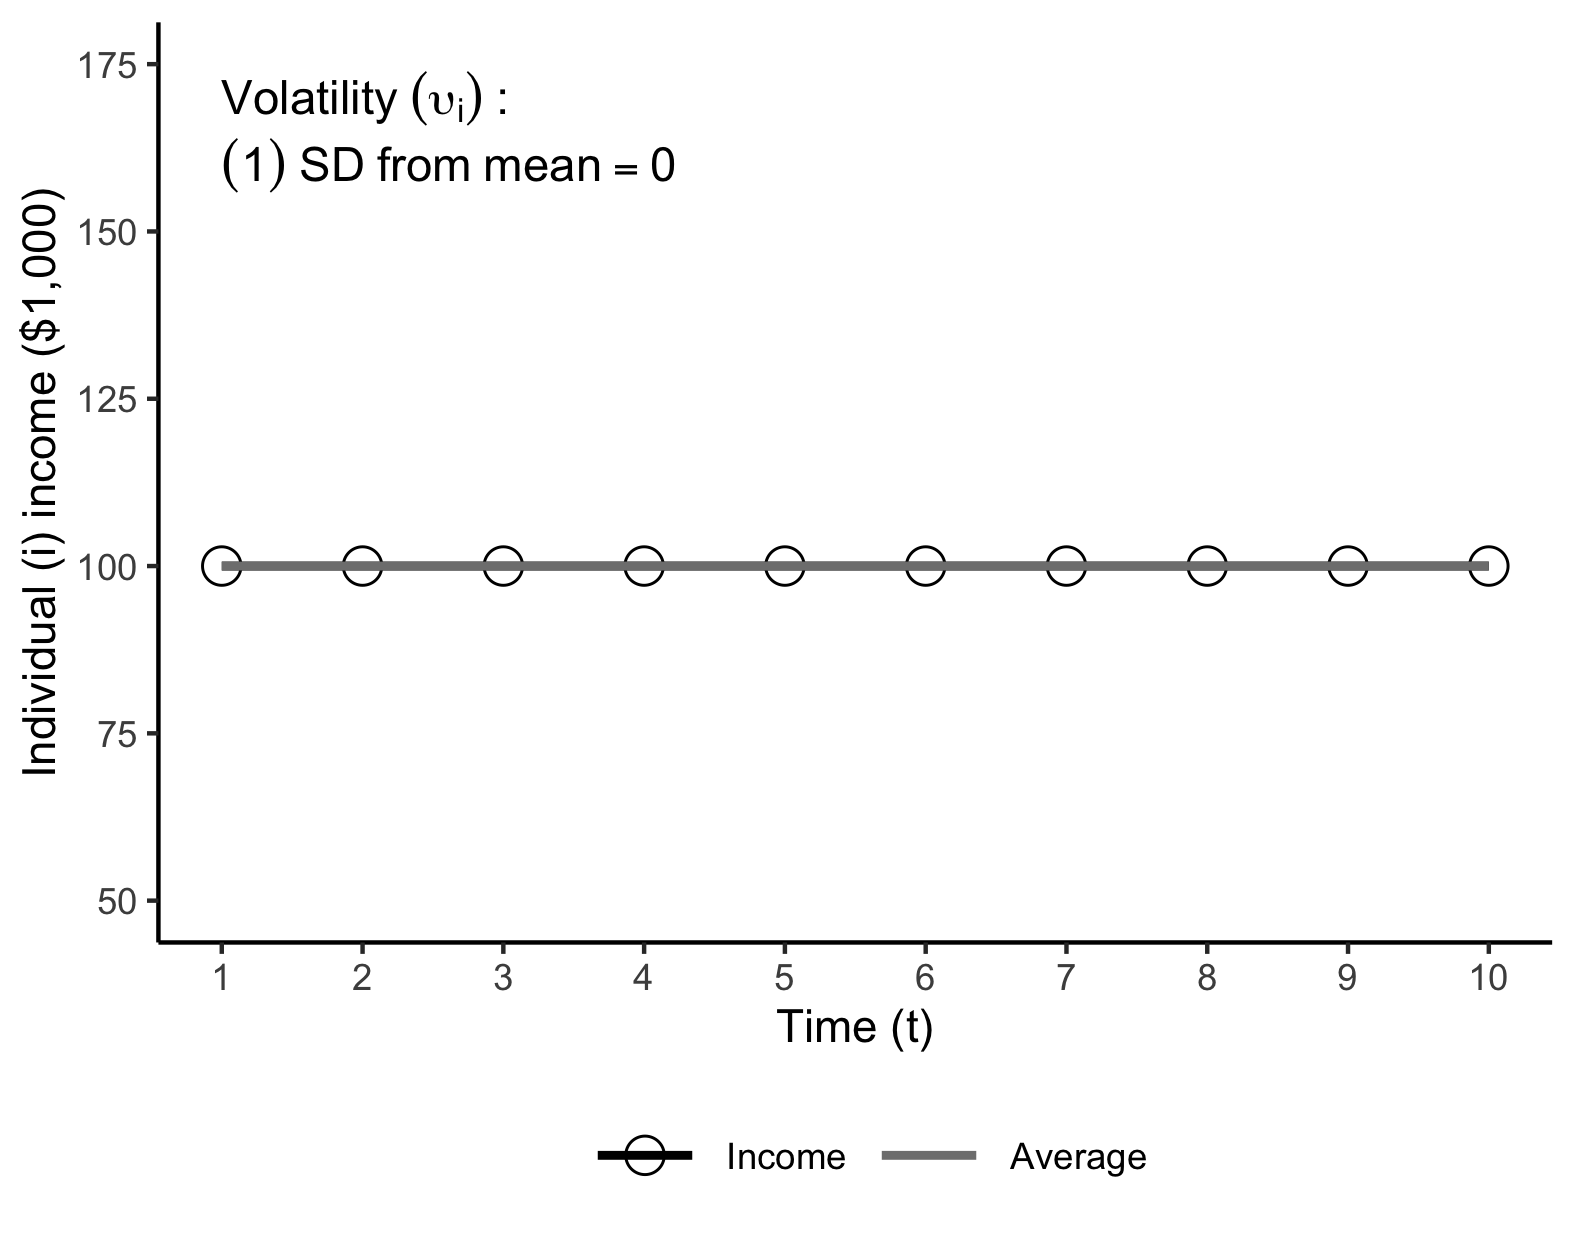
\includegraphics[width=\textwidth]{../graphs/example_1.png}
        \caption{No income change}
        \label{examples_sub1}
    \end{subfigure}
    \begin{subfigure}[b]{0.45\textwidth}
        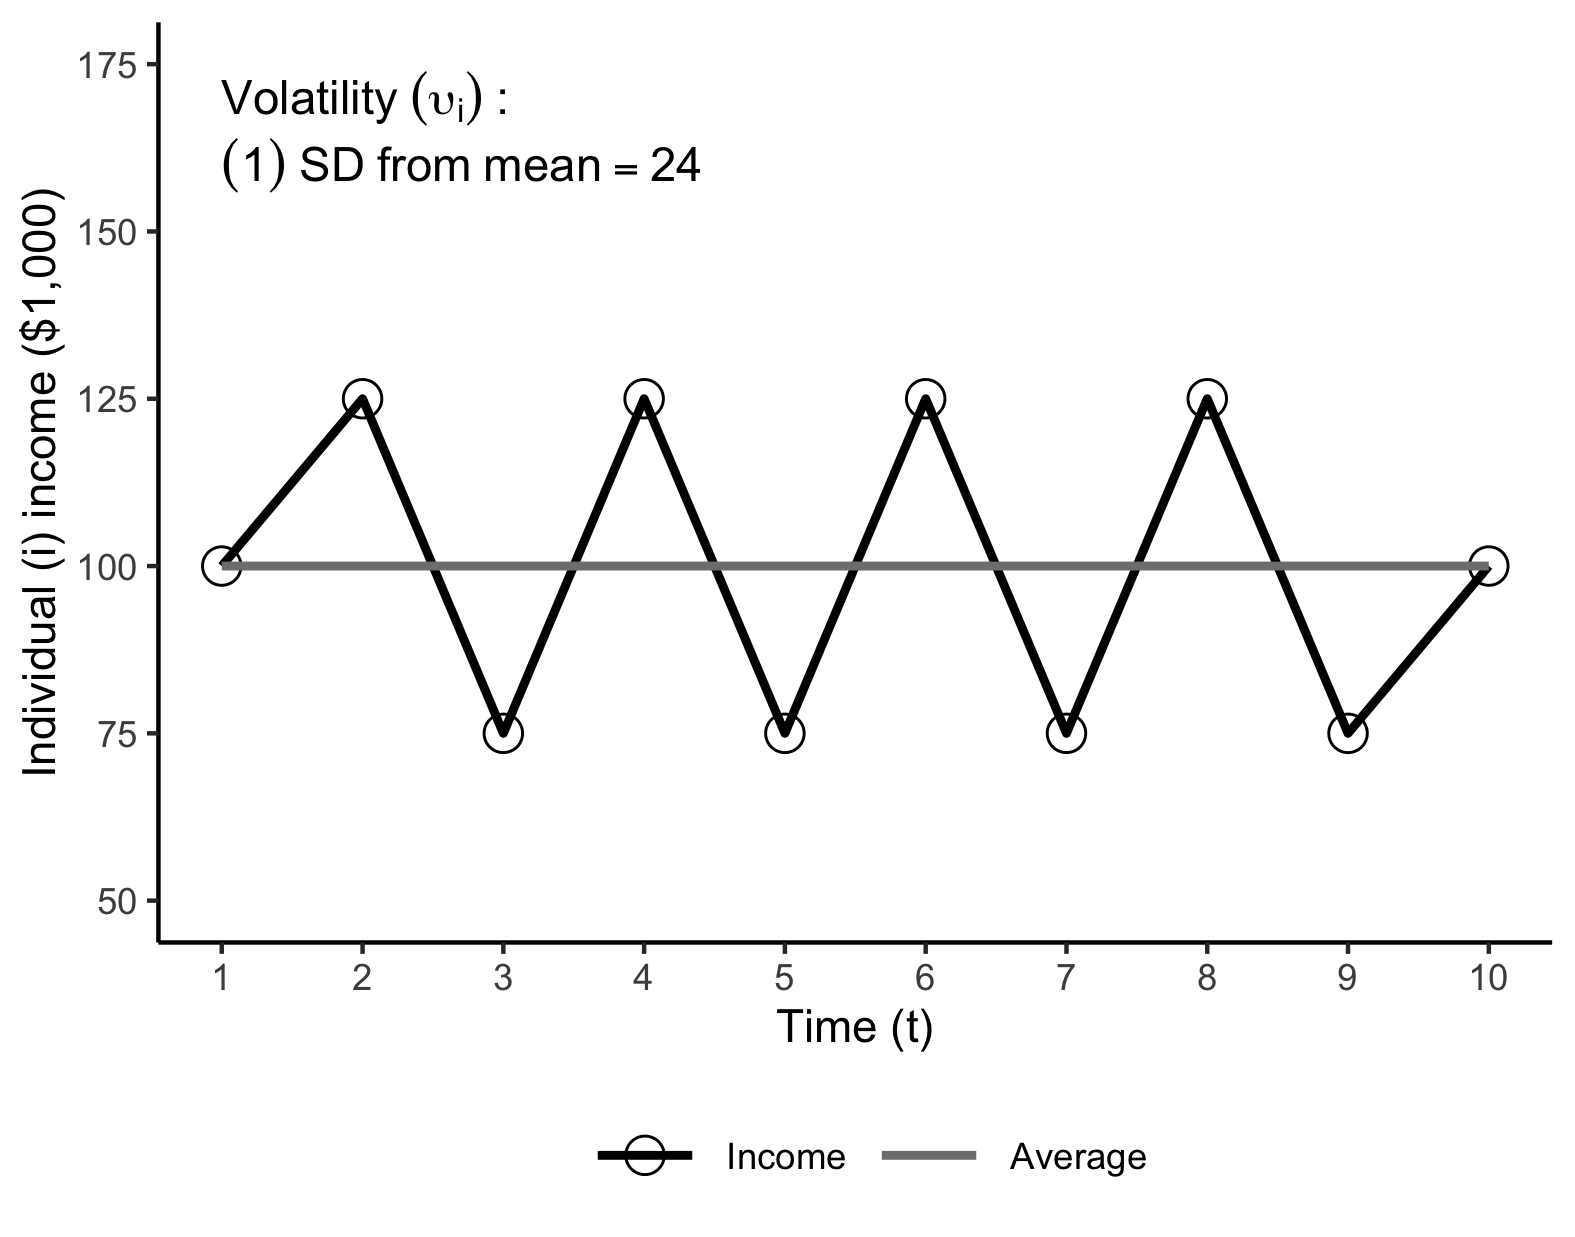
\includegraphics[width=\textwidth]{../graphs/example_2.png}
        \caption{Mean reverting}
        \label{examples_sub2}
    \end{subfigure}
        \begin{subfigure}[b]{0.45\textwidth}
        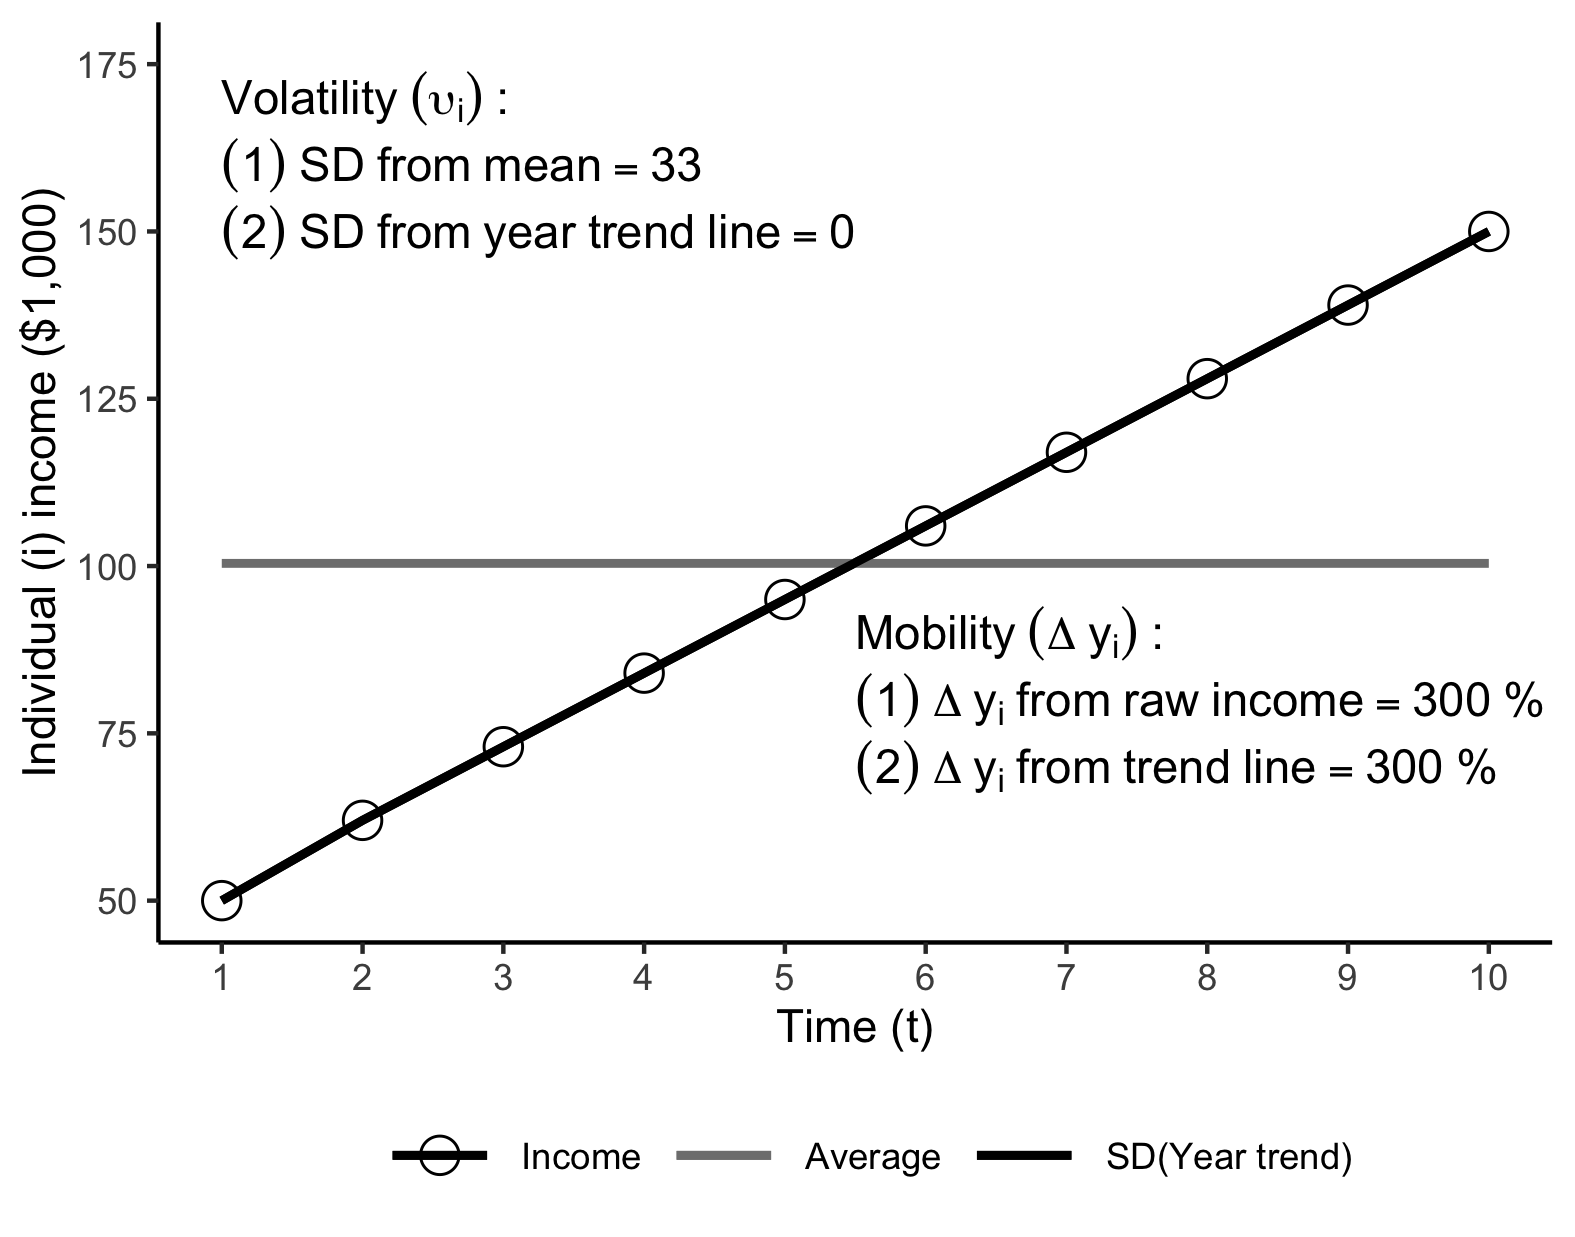
\includegraphics[width=\textwidth]{../graphs/example_3.png}
        \caption{Linear}
        \label{examples_sub3}
    \end{subfigure}
    \begin{subfigure}[b]{0.45\textwidth}
        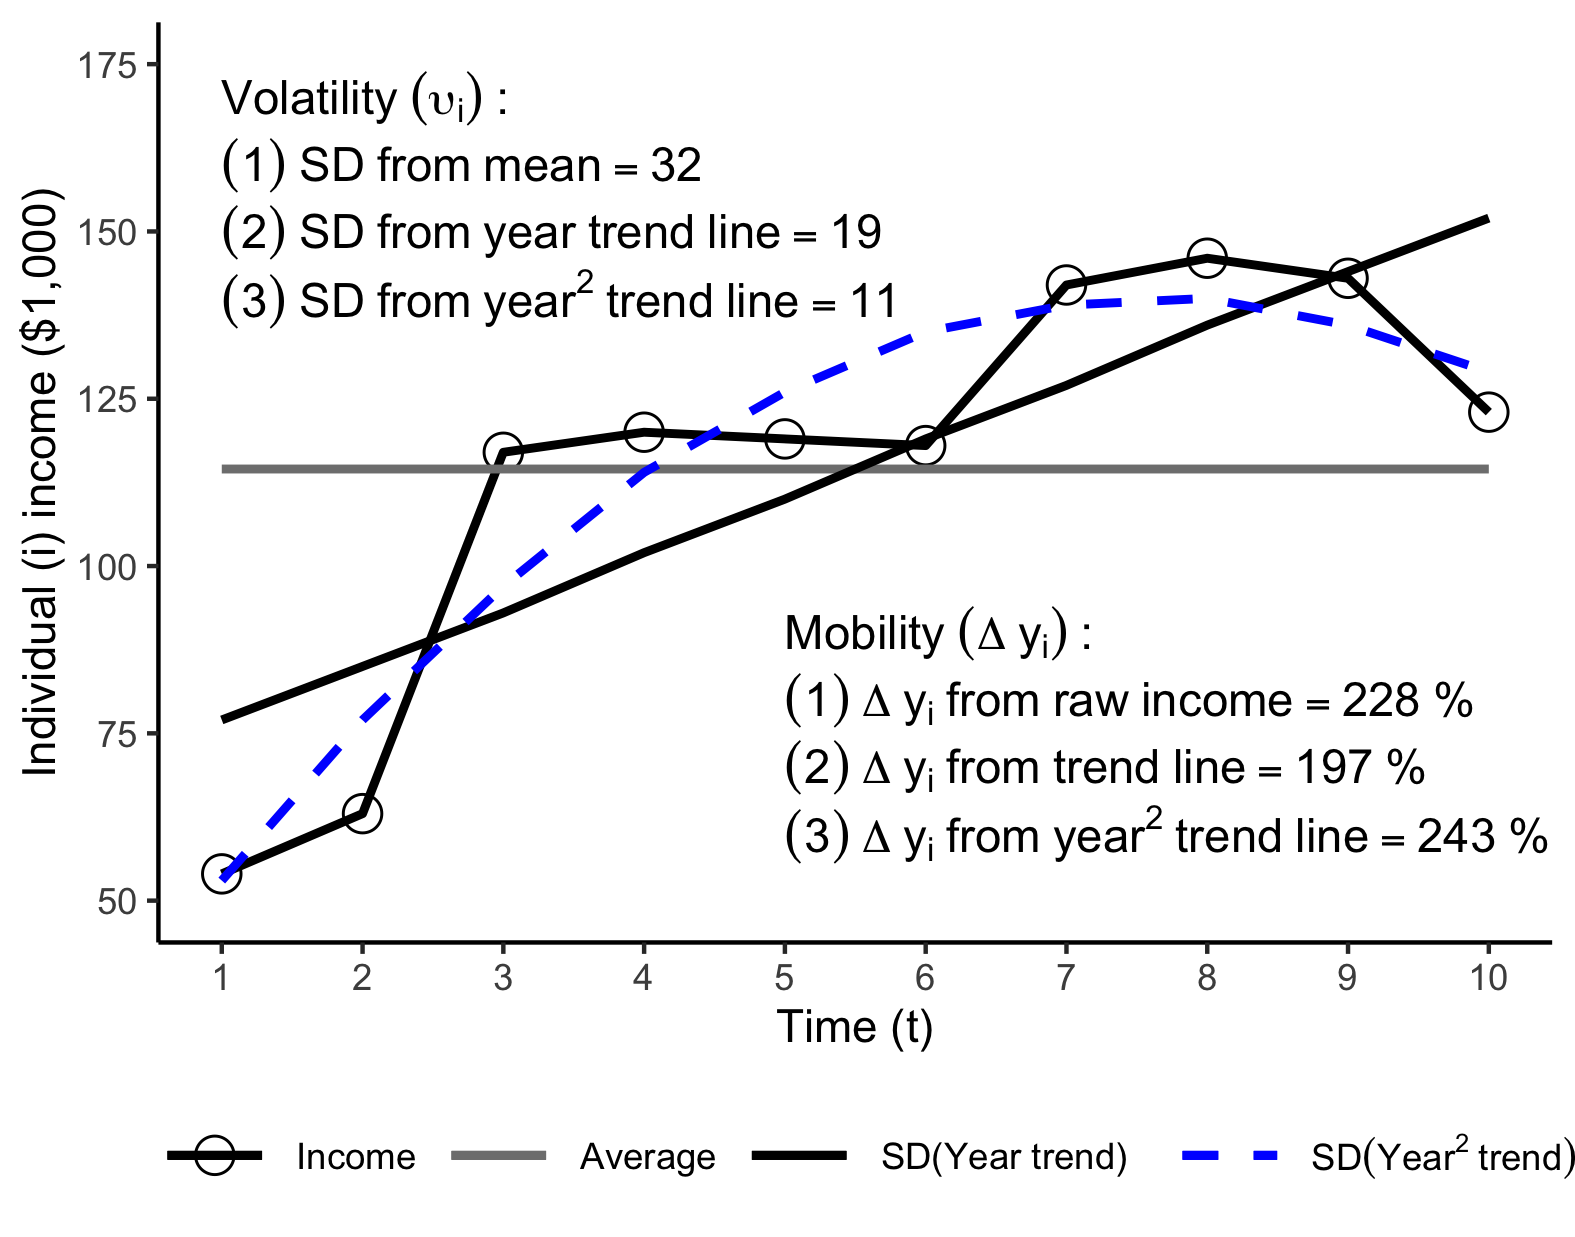
\includegraphics[width=\textwidth]{../graphs/example_psid.png}
        \caption{Curvilinear}
        \label{examples_sub4}
    \end{subfigure}
\end{figure}

\begin{figure}[htp!]
\centering
\caption{Income volatility over time with different measures of volatility} 
\centering
\resizebox{\textwidth}{!}{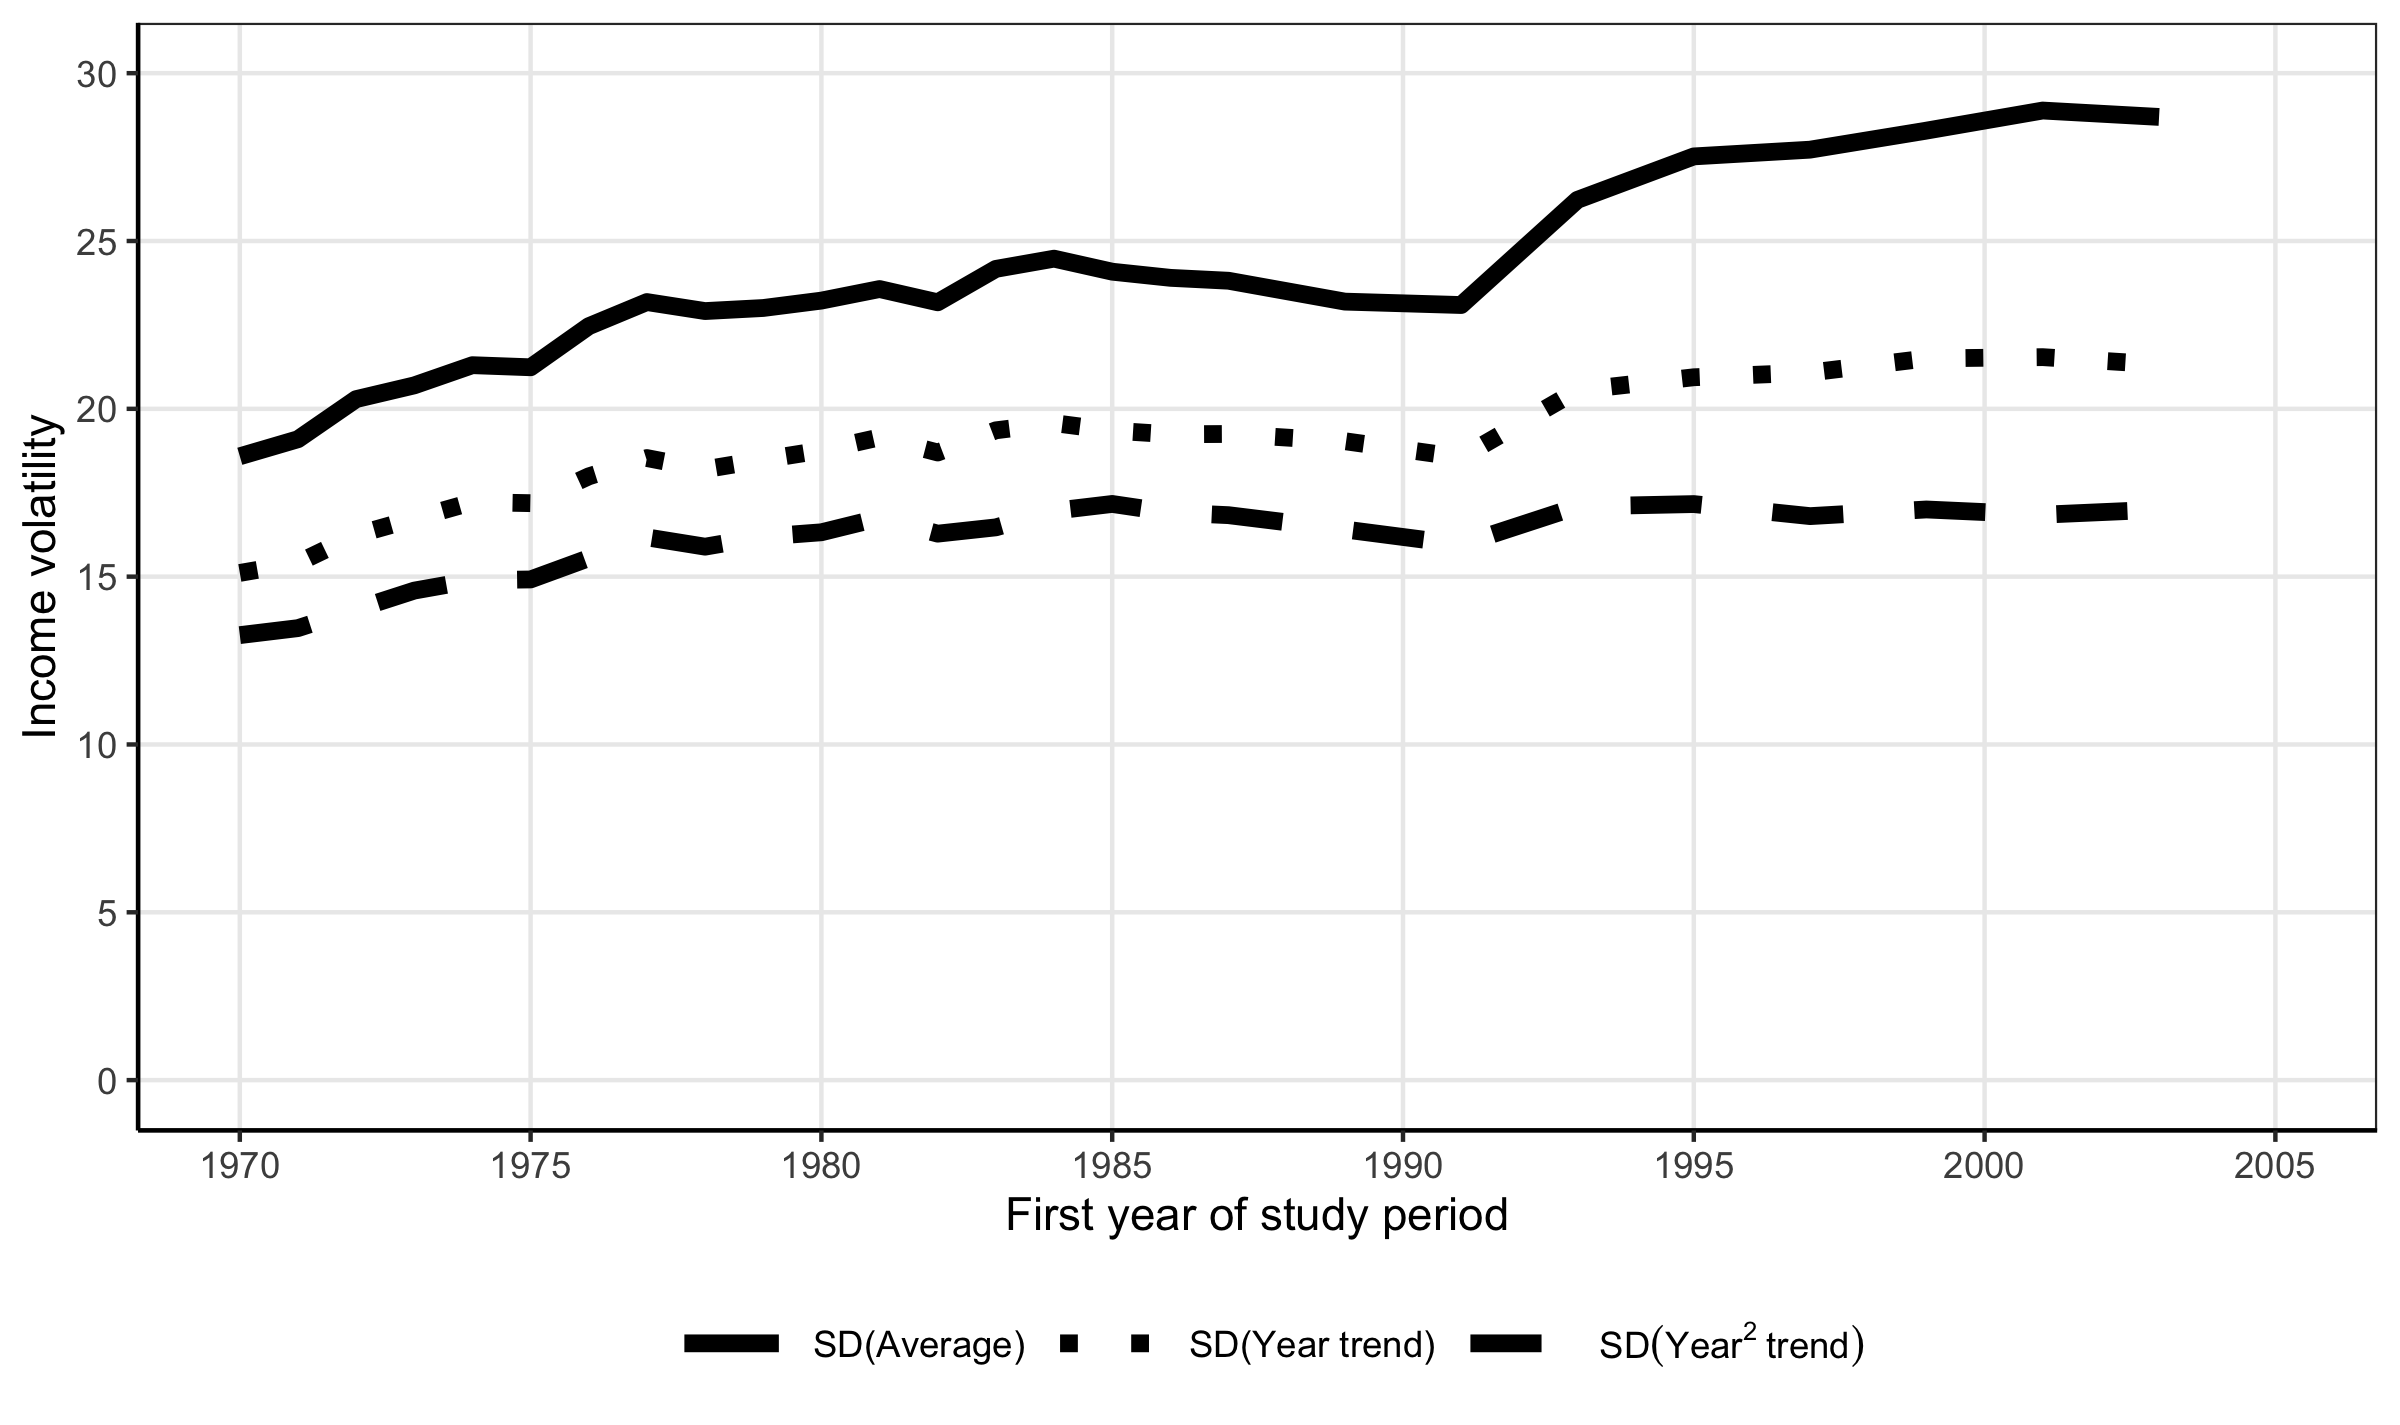
\includegraphics{../graphs/volatility_graph_src.png}}
\label{volatility_graph}
\end{figure}

\begin{figure}[htp!]
\centering
\caption{Predicted income volatility by income mobility from table \ref{regression}} 
\centering
\resizebox{\textwidth}{!}{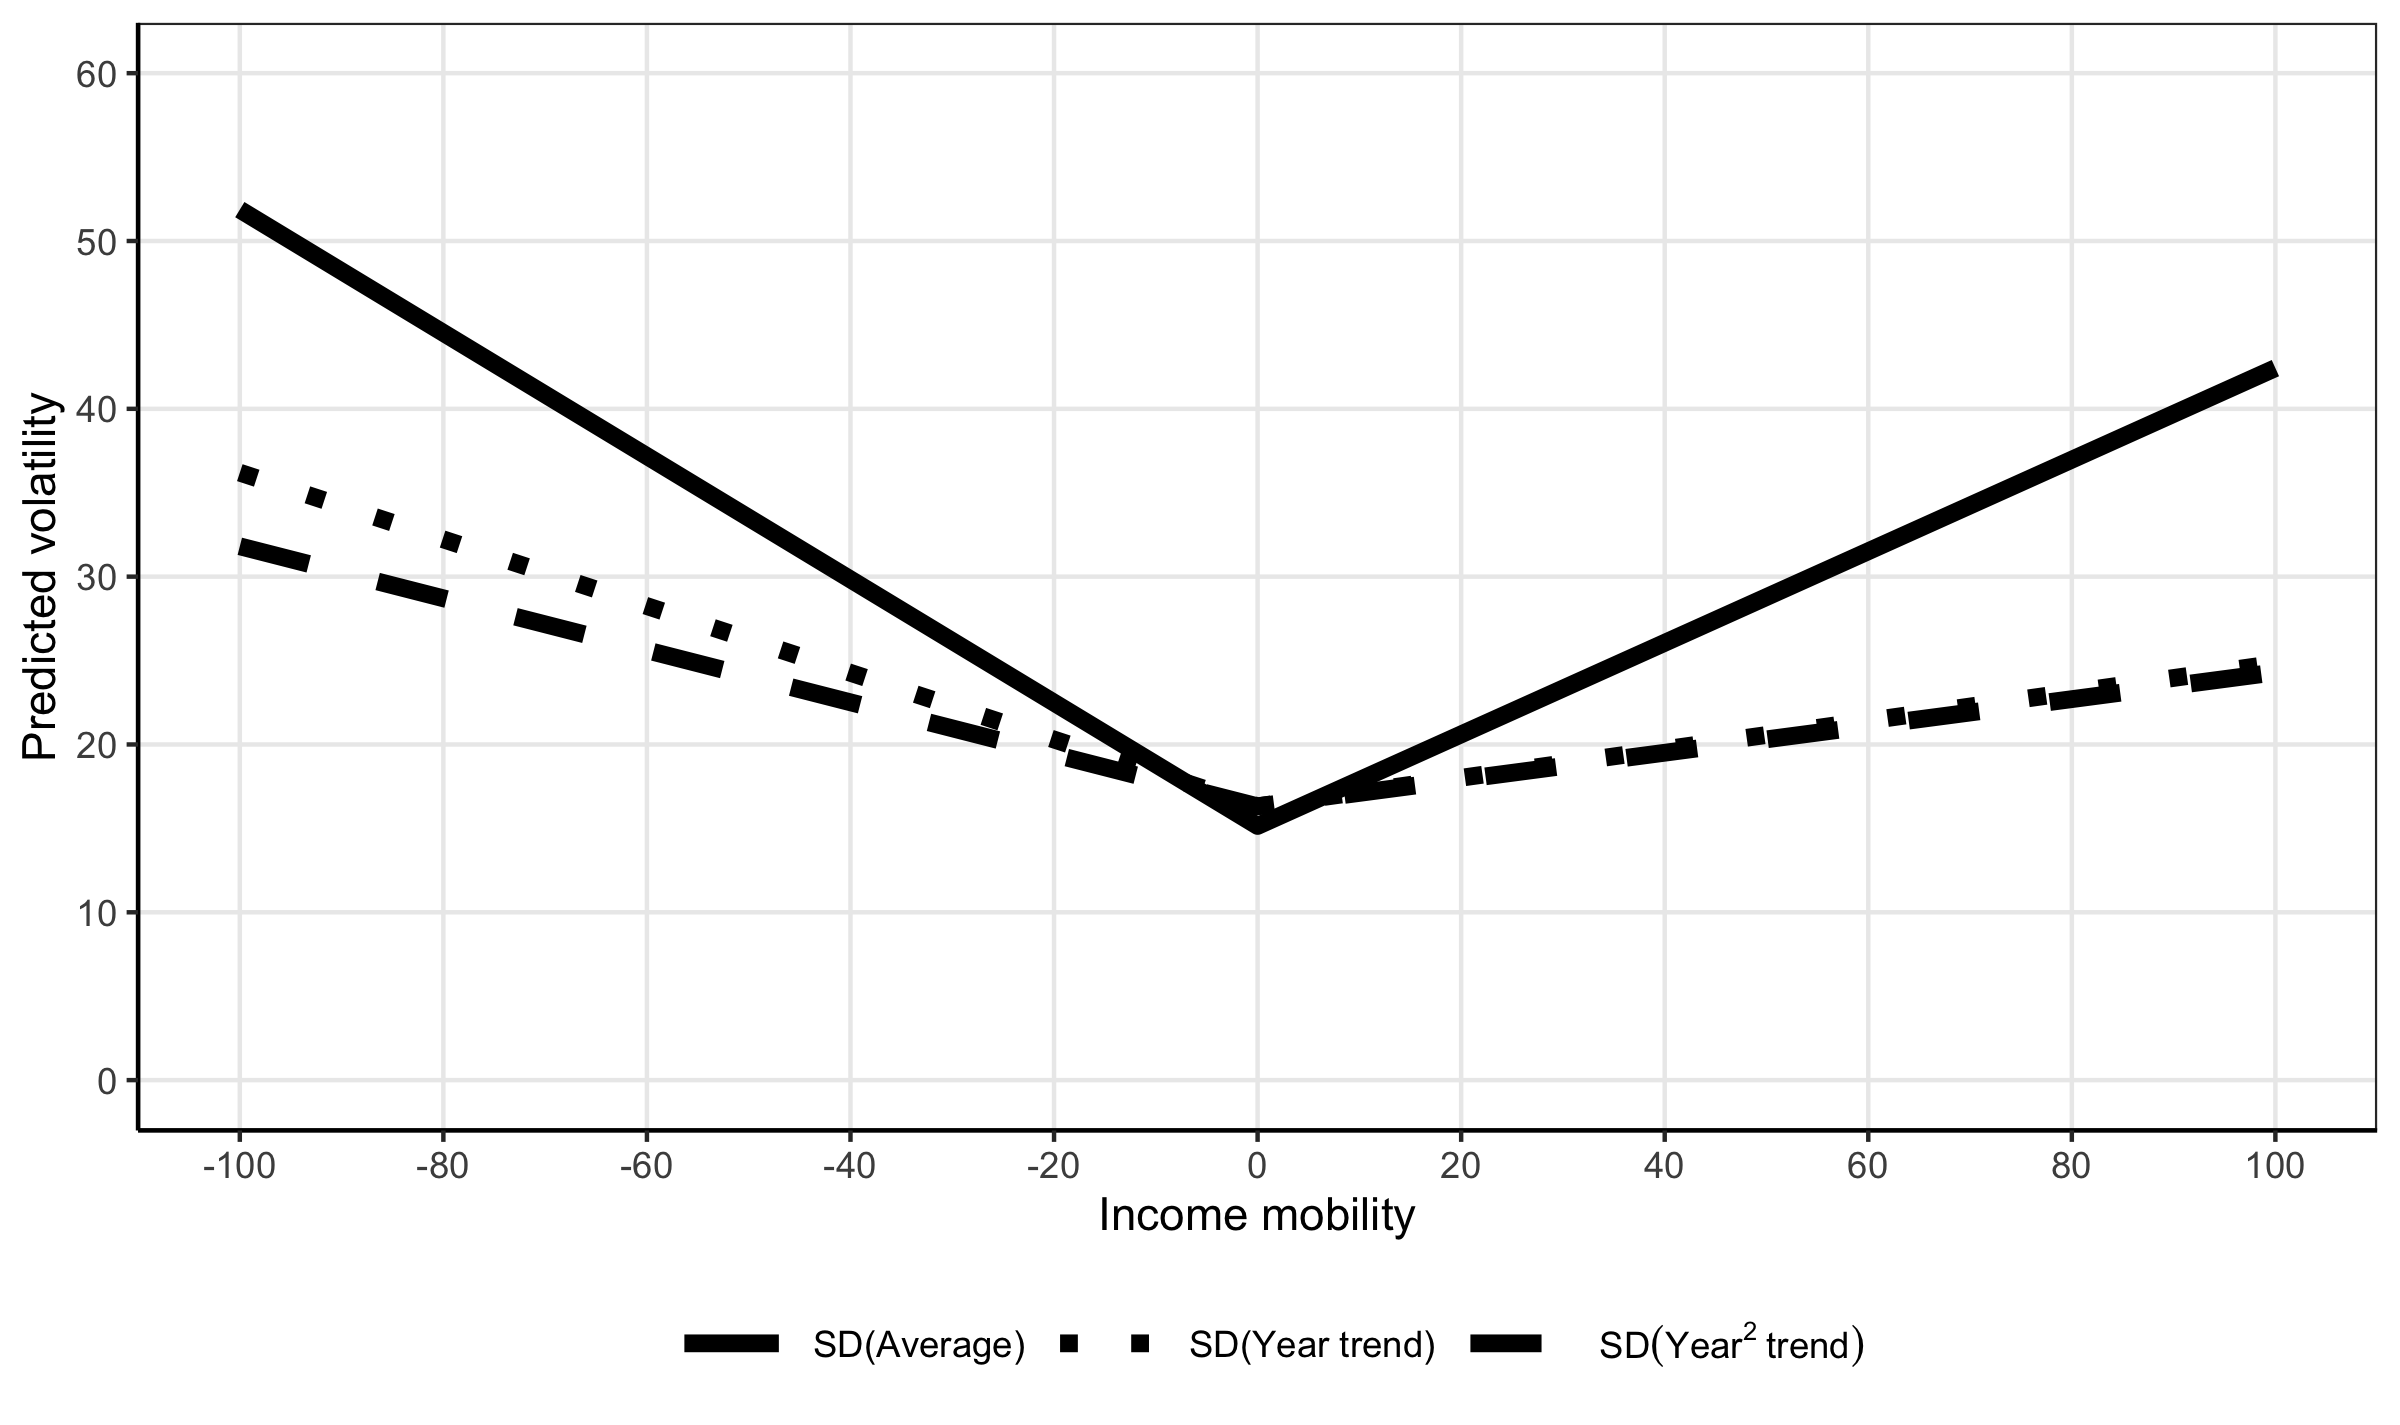
\includegraphics{../graphs/margins_ind_src_apc_w_o_cube.png}}
\label{margins_mobility}
\end{figure}

\end{document}

